\documentclass[12pt, openright, oneside, a4paper, brazil]{abntex2}
\usepackage{lmodern}
\usepackage[T1]{fontenc}
\usepackage[utf8]{inputenc}
\usepackage{nameref}
\usepackage[justification=justified,singlelinecheck=false]{caption}
\usepackage{lastpage}
\usepackage{amsmath}
\usepackage{indentfirst}
\usepackage{color}
\usepackage{graphicx}
\usepackage{microtype}
\usepackage[brazilian,hyperpageref]{backref}
\usepackage[alf, abnt-emphasize=bf, abnt-url-package=none, abnt-repeated-title-omit=yes, abnt-full-initials=yes, abnt-etal-list=3, abnt-etal-text=emph]{abntex2cite}
\usepackage{trabalho}
\usepackage{lipsum}
\usepackage{trivfloat}
\usepackage{listings}
\usepackage{xcolor}
\usepackage{caption}

% ---
% DEFINIÇÃO DE CORES
% ---

\definecolor{codegreen}{rgb}{0,0.6,0}
\definecolor{codegray}{rgb}{0.5,0.5,0.5}
\definecolor{codepurple}{rgb}{0.58,0,0.82}
\definecolor{backcolour}{rgb}{0.95,0.95,0.92}

% ---
% CONFIGURAÇÕES DE PACOTES
% ---

\lstdefinestyle{custompython}{
	backgroundcolor=\color{backcolour},
    commentstyle=\color{codegreen},
    keywordstyle=\color{codegreen},
    numberstyle=\tiny\color{codegray},
    stringstyle=\color{codepurple},
    basicstyle=\footnotesize,
    breakatwhitespace=false,
    breaklines=true,
    captionpos=b,
    keepspaces=true,
    numbers=left,
    numbersep=5pt,
    showspaces=false,
    showstringspaces=false,
    showtabs=false,
    tabsize=2
}

\trivfloat{quadro}
\renewcommand{\listquadroname}{Lista de Quadros}
\renewcommand{\backrefpagesname}{Citado na(s) página(s):~}
\renewcommand{\backref}{}
\renewcommand*{\backrefalt}[4]{
	\ifcase #1 %
		Nenhuma citação no texto.%
	\or
		Citado na página #2.%
	\else
		Citado #1 vezes nas páginas #2.%
	\fi}%

\titulo{UMA API REST ORIENTADA A METADADOS COMO SERVIÇO DE RECOMENDAÇÃO HÍBRIDA}
\autor{Iury Krieger}
\local{\vfill Videira - Santa Catarina}
\data{2017}
\orientador{Msc. Tiago Heineck}
\coorientador{Msc. Wanderson Rigo}
\instituicao{
  Instituto Federal Catarinense - Campus Videira
  \par
  Bacharelado em Ciência da Computação
}
\tipotrabalho{Trabalho de conclusão de curso}
\preambulo{
	Trabalho de conclusão de curso submetido ao Instituto Federal Catarinense - Campus Videira como parte dos requisitos para a obtenção do grau de Bacharel em Ciência da Computação
}
\makeatletter
\hypersetup{
	pdftitle={\@title},
	pdfauthor={\@author},
	pdfsubject={\imprimirpreambulo},
	pdfcreator={LaTeX with abnTeX2},
	pdfkeywords={abnt}{latex}{abntex}{abntex2}{trabalho acadêmico},
	colorlinks=true,       		% false: boxed links; true: colored links
	filecolor=magenta,      		% color of file links
	urlcolor=blue,
	bookmarksdepth=4
}
\makeatother
\setlength{\parindent}{1.3cm}
\setlength{\parskip}{0.2cm}
\makeindex

\begin{document}
\frenchspacing
\imprimircapa
\imprimirfolhaderosto

\begin{comment}
\begin{folhadeaprovacao}
	\begin{figure}[htb]
		\begin{center}
			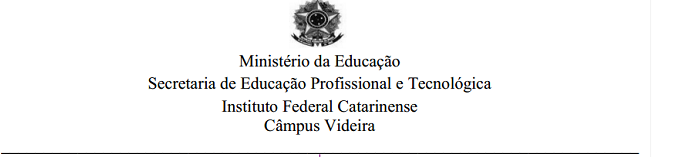
\includegraphics{images/logo.png}
		\end{center}
	\end{figure}
	{\ABNTEXchapterfont\large{\textbf{BACHARELADO EM CIÊNCIA DA COMPUTAÇÃO}}}
	\begin{center}
		{\ABNTEXchapterfont\large\imprimirautor}

		\vspace*{\fill}\vspace*{\fill}
		\begin{center}
			\ABNTEXchapterfont\bfseries\Large\imprimirtitulo
		\end{center}
		\vspace*{\fill}
	\end{center}

	Este Trabalho de Conclusão de Curso foi julgado adequado para a obtenção do título de Nome do Título em Nome do Curso, Área de Concentração e aprovada em sua forma final pelo Curso de Nome do Curso

	\assinatura{\textbf{\imprimirorientador} \\ Orientador}
	\assinatura{\textbf{Msc. Marcelo Cendron} \\ Professor Convidado I}
	\assinatura{\textbf{Maurício Ferreira} \\ Professor Convidado II}

	\begin{center}
		\vspace*{0.5cm}
		{\large\imprimirlocal}
		\par
		{\large\imprimirdata}
		\vspace*{1cm}
	\end{center}
\end{folhadeaprovacao}
\end{comment}

\begin{folhadeaprovacao}

  \begin{center}
  \vspace*{-1.2cm}
    {\large\imprimirautor}

    \vspace*{\fill}\vspace*{\fill}\vspace*{\fill}
    {\large\imprimirtitulo}
    \vspace*{\fill}\vspace*{\fill}

    \hspace{.45\textwidth}
    \begin{minipage}{.5\textwidth}
        \imprimirpreambulo
    \end{minipage}%
    \vspace*{\fill}
   \end{center}

  \begin{center}
  	 Videira (SC), 16 de Maio de 2017
  \end{center}

    \vspace{-1cm}

   \assinatura{\begin{center}\vspace{-0.6cm}\imprimirorientador \\
   					   Instituto Federal Catarinense
   					   \end{center}
   	}
   	\assinatura{\begin{center}\vspace{-0.6cm} Msc. Wanderson Rigo \\
   					   Instituto Federal Catarinense
   					   \end{center}
   	}
    \begin{center}
  	\textbf{BANCA EXAMINADORA}
   \end{center}
   \vspace{-1cm}
   \assinatura{\begin{center}\vspace{-0.6cm} Msc. Marcelo Cendron \\
      					   Instituto Federal Catarinense
   					     \end{center}
   }
   \assinatura{\begin{center}\vspace{-0.6cm}Maurício Ferreira \\
       					   Instituto Federal Catarinense
   					    \end{center}
    }

    \vspace*{1cm}

\end{folhadeaprovacao}

\begin{dedicatoria}
	\vspace*{\fill}
	\centering
	\noindent

	\textit{Aos meus pais, professores, mentores, amigos e todas as pessoas que, de alguma maneira, possibilitaram que minha pessoa chegasse até aqui, na forma do meu mais profundo agradecimento, dedico-vos a existência deste trabalho.}

	\vspace*{\fill}
 \end{dedicatoria}

\setlength{\absparsep}{18pt} % ajusta o espaçamento dos parágrafos do resumo
\begin{resumo}

Devido a expansão massiva de dados produzidos e disponíveis na Internet, os usuários estão cada vez mais sobrecarregados de informação, não sabendo distinguir informações realmente úteis. Para sanar este problema, os sistemas de recomendação visam recomendar os itens mais úteis a cada usuário, através de técnicas de \textit{machine learning}. Tais técnicas visam prever a avaliação de um usuário a um item, baseando-se nas avaliações já conhecidas. Este trabalho propõe o desenvolvimento de uma API REST de código aberto que recomenda itens a usuários, fazendo uso de um sistema de recomendação híbrido que analisa as estruturas de metadados pré definidas e proporciona recomendações, através do conteúdo do item e da filtragem colaborativa de usuários. Dessa forma é possível fornecer um serviço multipropósito, totalmente personalizável, trazendo uma visão mais precisa dos sistemas de recomendação aos desenvolvedores.

\textbf{Palavras-chaves}: Sistemas de Recomendação. Aprendizado de Máquina. Metadados.
\end{resumo}

\begin{resumo}[Abstract]
\begin{otherlanguage*}{english}

Due to the massive expansion of data produced and available on the Internet, users are increasingly overloaded with information, not knowing how to distinguish really useful ones. To remedy this problem through machine learning techniques, the recommendation systems aim to recommend the most useful items to each user. Such techniques are intended to predict a user's rating of an item, based on previously known ratings. This work proposes the development of a REST Open Source API that recommends items to users, making use of a hybrid recommendation system that analyzes pre-defined metadata structures and provides recommendations through item content and collaborative user filtering. In this way it is possible to provide a fully customizable multipurpose service, bringing a more accurate view of the recommendation systems to developers.

\textbf{key-words}: Recommender Systems. Machine Learning. Metadata.
\end{otherlanguage*}
\end{resumo}

% ---
% Lista de quadros
% ---
\counterwithout{quadro}{chapter}
\newpage % Forçar a lista de quadros em uma nova página
\phantomsection % Comando necessário caso o pacote hyperref seja utilizado, visando a corrigir o link
\pdfbookmark[0]{\listofquadros}{lof}
\listofquadros* % Adiciona lista de quadros
\cleardoublepage

% ---
% Lista de figuras
% ---
\pdfbookmark[0]{\listfigurename}{lof}
\listoffigures*
\cleardoublepage

% ---
% Siglas
% ---
\begin{siglas}

	\item[IA]{\textit{Inteligência Artificial}}
	\item[HTTP]{\textit{Hypertext Transfer Protocol}}
	\item[URI]{\textit{Uniform Resource Identifier}}
	\item[XML]{\textit{eXtensible Markup Language}}
	\item[HTML]{\textit{HyperText Markup Language}}
	\item[API]{\textit{Application Program Interface}}
	\item[REST]{\textit{Representational State Transfer}}
	\item[JSON]{\textit{Javasript Object Notation}}
	\item[IP]\textit{Internet Protocol}

\end{siglas}

% ---
% Sumário
% ---
\pdfbookmark[0]{\contentsname}{toc}
\tableofcontents*
\textual

\chapter{INTRODUÇÃO} \label{intro}

Com o avanço crescente do campo tecnológico, os computadores vêm desempenhando tarefas antes incumbidas à seres humanos. O poder de computação provou-se muito eficaz ao desempenhar tarefas que possuíssem um padrão possível de se expressar através de um algoritmo, mais ainda, se este padrão fosse repetitivo.

Logo os computadores começaram a desempenhar funções nas mais diversas áreas, desde cálculos matemáticos à manipulação de imagens. Atualmente, das funções desempenhadas pelos computadores, a mais difícil de se reproduzir com precisão é o padrão de raciocínio humano.

Alguns autores defendem que para que um computador atinja tal nível, seria necessário que o mesmo possuísse consciência, assim como os seres humanos. Outros defendem que o raciocínio humano não consegue ser reproduzido, apenas emulado, devido à impossibilidade de se programar uma consciência computacional. Tal área de estudo, que tem como o foco o desenvolvimento de sistemas computacionais rumo a proximidade do método humano, chama-se inteligência artificial \cite{russell2004inteligencia, coppin2015inteligencia}.

Possível ou não, é inegável o avanço da inteligência artificial desde seu início nos primórdios da computação. Algumas tarefas, tais como a atribuição de uma consciência a um sistema computacional, deixaram de ser o foco da área, uma vez que não possuímos a tecnologia para construir sistemas muito mais complexos que os atuais  \cite{russell2004inteligencia}.

Entretanto, a inteligência artificial encontrou-se muito eficaz em outras áreas do método humano, tais como o aprendizado, um dos segmentos mais importantes da área, dentro da inteligência artificial chamado de aprendizado de máquina (\textit{machine learning}) \cite{coppin2015inteligencia}.

Desde os anos 90 a preocupação com o armazenamento e a expansão massiva de dados produzidos já existia, prevendo que usuários ficariam sobrecarregados de informação, não sabendo distinguir o que seria realmente útil \cite{hill1995recommending, adomavicius2005toward}. Na época, uma comunidade virtual de avaliação foi proposta para proporcionar aos usuários o mínimo de esforço ao encontrar informações úteis. Com a evolução da inteligência artificial e das técnicas de machine learning, este trabalho de avaliação e recomendação, antes feito por uma comunidade, hoje é atribuído aos sistemas de recomendação \cite{hill1995recommending}.

Sistemas de recomendação (RSs) são ferramentas de  software e técnicas que provém sugestões de artefatos à usuários. Estes artefatos são definidos como os objetos de valor à serem recomendados \cite{ricci2011introduction}. Atualmente, o interesse em tais sistemas se mantém alto, devido a abundância de aplicações práticas \cite{adomavicius2005toward}, exemplificadas nos casos de \textit{E-commerce} por \citeonline{schafer2001commerce}, além de \citeonline{linden2003amazon}, onde são amplamente utilizados.

Desta forma, sistemas de recomendação vem sendo desenvolvidos para a resolução do problema descrito nas mais diversas áreas \cite{bennett2007netflix, gavalas2014mobile}, desde aplicações hoteleiras como o TripAdvisor até aplicações de entretenimento como a Netflix, além da sua origem nos \textit{E-commerces} citados anteriormente. Muitos destes sistemas são casos de RSs aplicados a itens e finalidades específicas \cite{huang2002graph, brozovsky2007recommender}, onde todo o motor de recomendação segue uma abordagem baseada no padrão que lhe foi dado.

Por outro lado, ao observar aplicações web de sistemas de recomendação, verifica-se a existência de soluções em forma de APIs, tais como o Google Cloud Platform e o Microsoft Cognitive Services, fornecidas como serviços transparentes. Entretanto, estas soluções proprietárias não são incorporadas a aplicação, mas sim utilizadas como serviços externos, dificultando a personalização.

Para sanar estes problemas, este trabalho propõe o desenvolvimento de uma API que proporcione uma visão mais transparente dos sistemas de recomendação, permitindo ao usuário desfrutar das funcionalidades, sem a necessidade de um profundo conhecimento dos detalhes que compõem as diferentes técnicas de recomendação, além dos problemas decorrentes do uso de cada uma das técnicas. Além disso, tal tecnologia será fornecida como um serviço de código aberto, podendo ser utilizada em qualquer ambiente.

Este trabalho está dividido em seis seções. A segunda seção apresenta o referencial teórico necessário para o entendimento total do escopo do trabalho. Na terceira seção são apresentadas as principais características do trabalho proposto, além de compará-lo com outros trabalhos relacionados. Em seguida, a quarta seção apresenta a metodologia a ser utilizada para realização do trabalho proposto na seção anterior. Mais à frente, na seção cinco, será abordado o cronograma a ser empregado para a realização do trabalho e, por fim, na sexta seção são apresentadas as considerações finais.

\section{Objetivos} \label{objectives}

\subsection{Objetivo Geral}

Desenvolver uma API web de código aberto para recomendação híbrida de itens a usuários.

\subsection{Objetivos Específicos}

\begin{itemize}
	\item Fornecer uma documentação das funcionalidades visando futura colaboração da comunidade e utilização por outros desenvolvedores.

	\item Proporcionar a recomendação das propriedades relevantes através das estruturas de metadados fornecidas.
\end{itemize}

\section{Metodologia}

A metodologia deste trabalho está dividida em três seções. Primeiramente serão implementadas todas as funcionalidades descritas na seção \nameref{objectives}. Mais à frente, será feita a validação das funcionalidades implementadas e da eficácia das recomendações. Por fim, serão feitos os ajustes e correções necessárias de acordo com o resultado da validação das funcionalidades implementadas.

\subsection{Implementação}

Inicialmente serão implementados os algoritmos de recomendação híbrida, incluindo o processamento dos metadados fornecidos. Os algoritmos de recomendação resumem a eficácia da API e devem consumir a maior parte do tempo de desenvolvimento.

Ao completar a implementação das técnicas híbridas de sistemas de recomendação, serão implementadas as demais funcionalidades da API. Serão consideradas a identificação e entrada dos metadados, além do formato dos dados de saída.

\subsection{Validação}

Assim que a API esteja em um grau considerado funcional, será feita a validação da eficácia ao recomendar as estruturas fornecidas através de grupos de testes definidos, uma técnica amplamente utilizada na validação de técnicas de machine learning.

A validação será feita utilizando um grupo separado dos  dados utilizados para testes, confrontando as recomendações feitas com o resultado esperado. Através desses resultados é medida a acurácia de um sistema de recomendação, métrica utilizada como medida de eficiência entre os diferentes métodos utilizados.

\subsection{Ajustes e Correções}

Por fim, serão feitos os ajustes e correções de erros recolhidos ao longo do processo, além de testar as funcionalidades e a utilização da API como um todo. A documentação será feita durante boa parte de todo o processo e, neste caso em específico, possui um foco especial, uma vez que o princípio da API é que a mesma seja utilizável por outros desenvolvedores, além de possibilitar a contribuição da comunidade.

\section{Trabalhos Relacionados} \label{related_work}

Tendo como base as técnicas descritas acima, existem trabalhos como os apresentados por \citeonline{guo2015librec}, que abordam as técnicas em forma de biblioteca Java a ser incluída nos projetos. Esta abordagem torna a utilização mais simples devido ao fato do usuário poder utilizar apenas as funcionalidades da biblioteca, preocupando-se com o formato de entrada e saída dos dados, não com o processo de recomendação em si. Outra abordagem interessante é a proposta por \citeonline{brozovsky2007recommender} ao construir uma biblioteca C\# multipropósito, focando na recomendação de itens com base na avaliação em um esquema de \textit{rating} (de uma a cinco estrelas), ou com base apenas em itens com avaliação positiva.

Em relação ao trabalho acima citado, a API proposta neste trabalho também visa ser multipropósito e distribuída como código aberto pela licença pública GNU (\textbf{GPL}), porém, fornecendo tais funcionalidades como um serviço web independente de linguagem de programação, o que não acontece nos exemplos apresentados.

Além dos trabalhos apresentados, \citeonline{do2013filtragem} aborda os sistemas de recomendação com uma perspectiva semelhante a este trabalho, focando mais no ganho de desempenho ao processar o método de filtragem colaborativa na GPU. Este trabalho não tem seu foco em desempenho, mas sim em uma proposta de \textbf{recomendação genérica}, que forneça recomendações a quaisquer modelos de usuários e itens através do método híbrido.

%
%--------- FIM INTRODUÇÃO------------
%

\cleardoublepage



\postextual

\bibliography{referencias}



\end{document}